\documentclass[a4paper,10pt,oneside]{article}
\usepackage[polutonikogreek,italian]{babel}
\usepackage[utf8x]{inputenc}
\usepackage{amsmath}
\usepackage{amsthm}
\usepackage{amssymb}
\usepackage{amscd}
\usepackage[pdftex,colorlinks=true,urlcolor=black]{hyperref}
\usepackage{graphicx}
\usepackage{float}
\usepackage{array}
\usepackage{rotating}
\usepackage[small]{caption}
\usepackage{lscape}
\usepackage{fancybox}
\usepackage{booktabs}
\usepackage[noanswer]{exercise}
\parindent0ex
\renewcommand{\fboxsep}{0.4cm}
\renewcommand{\textfraction}{0.05}
\renewcommand{\topfraction}{0.95}
\renewcommand{\bottomfraction}{0.95}
\renewcommand{\floatpagefraction}{0.35}
\renewcommand{\ExerciseName}{Esercizio}
\renewcommand{\ExerciseListName}{Es}
\setcounter{totalnumber}{5}
\restylefloat{figure}
\begin{document}
\section*{Gli eventi nello spazio}
\begin{figure}[H]
 \centering
 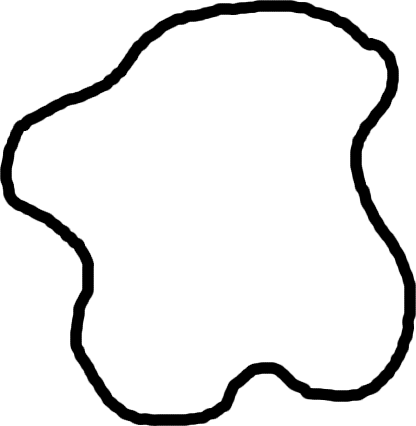
\includegraphics[width=.7\textwidth]{../immagini/superficieIrregolare.png}
 % superficieIrregolare.png
 \label{fig:superficieIrregolare}
\end{figure}


\subsection*{Fisica e geometria}
I fenomeni naturali osservati dalla fisica sono eventi immersi nello spazio e nel tempo.
In particolare, lo spazio è forse il primo elemento di cui si è occupata la fisica almeno dai tempi dei filosofi greci.

Ai giorni nostri, invece, la descrizione dello spazio è affidata piuttosto alla geometria, considerata come una branca
della matematica.
La geometria è una disciplina che studia un insieme di eventi astratti, chimati punti, linee, superfici, volumi e via
dicendo. Nessuno di questi enti possiede una porpria definizione fisica. La geometria, infatti, non dichiara mai cosa
sono gli enti di cui si occupa, ma descrive soltanto le loro proprietà. Che cos'è, ad esempio, un punto o una retta?

Non ha importanza. In geometria basta sapere  che esistono infiniti punti e che per due punti passa una e una sola
retta.

La fisica, invece, osserva degli oggetti reali e, se del caso, attribuisce ad essi le proprietà degli enti geometrici.
I filosofi greci, ad esempio, costruivano dei semicerchi con un compasso sulla sabbia, poi si procuravano una fettucia
flessibile e la riportavano lungo la semicirconferenza. Riproducendo l'esperienza con cerchi di raggio differente,
osservavano che il raggio è contenuto sempre tre volte nel prorpio semicerchio, con un piccolo resto. Dunque per loro il
pigreco non era una proprietà matematica della circonferenza, ma il risultato di un'evidenza sperimentale.

Per questo motivo, i greci si impegnavano moltissimo per dare una definizione concreta agli enti astratti. Noi, oggi,
qualche volta, facciamo addirittura il contrario. In un problema, ad esempio, può capitare di rappresentare come un
punto un'autocorriera che trasporta 60 passeggeri in viaggio sull'autostrada. Ma questa scelta potrebbe rivelarsi
inadatta se è necessario descrivere la corriera mentre affronta un tornante su una strada di montagna.

Pensiamo allora a quante volte ci capita di sostituire l'oggetto che stiamo osservando con un ente geometrico astratto.
Che cos'è, ad esempio, una retta? A seconda delle situazioni, può essere un righello, un filo sottile ben teso, il
bordo della lavagna o la scia di un aeroplano.

Albert Einstein ha proposto di utilizzare, come modello di retta, il percorso di un raggio di luce. Durante
l'osservazione di un eclisse di sole, è stato osservato che, sebbene il disco solare possieda un diametro angolare più
piccolo della Luna, alcuni raggi di luce riescono comunque a raggiungere la terra proprio nell'epicentro
dell'eclisse, come se avessero la capacità di girarle attorno. Comportamenti analoghi sono stati osservati per alcune
stelle lontane, nascoste da altre più vicine alla terra.

Riflettendo un attimo, possiamo accorgeci che un raggio di luce capace di raggiungere la terra girando attorno alla
Luna, può scegliere ad arbitrio molti percorsi diversi, contro il postulato secondo il quale per due punti passa una e
una sola retta. Da questa osservazione si è dedotto, perciò, che in particolari condizioni, le rette possono avere
proprietà geometriche differenti da quelle che siamo abituati a usare. Ed Albert Einstein ha ricavato da questo
fenomeno una conferma della Teoria della Relatività Generale.

\subsubsection*{Il piano Cartesiano}

La scomposizione di un vettore può avvenire usando un qualunque sistema di assi, ma è comodo usare una coppia di {\bfseries rette ortogonali}. Se invece si lavora sull'insieme dei punti dello spazio, sarà necessario usare tre direttrici, che prendono il nome di {\bfseries terna cartesiana} \footnote{oppure terna ortogonale}.\newline
un sistema di assi cartesiani conferisce allo spazio una struttura di riferimento, che è molto utile nella rappresentazione dei vettori.
 
Ogni vettore $ \vec{v}$ del piano, infatti, può essere scomposto in un modo unico in due componenti, in modo che sia:
\begin{center}
\begin{math}
\vec {v} = \vec{v_x} + \vec{v_y}
\end{math}
\end{center}
Ciascuna componente di un dato vettore è, a sua volta un vettore, la cui intensità è determinata in funzione di una corrispondente unità di misura.\newline
Su ciascun asse cartesiano, pertanto, viene definito un vettore unitario, detto {\bfseries versore}.
Comunemente, i versori dello spazio tridimensionale sono indicati dalle lettere
$\vec i$,$\vec j$ e ${\vec k}$. Si può scrivere dunque:
\begin{center}
\begin{equation}\label{eq:scomposizioneDiUnVettore}
\vec v = v_x \vec i + v_y \vec j
\end{equation}
\end{center}

Usare il piano cartesiano rende più semplici le operazioni di somma e differenza. Infatti è possibile operare separatamente sulle componenti cartesiane indipendenti, come nel seguente esempio:
\begin {center}
\begin{math}
\vec v \pm \vec u = (v_x \vec i \pm v_y \vec y) + (u_x \vec i \pm u_y \vec j) = (v_x \pm u_x) \vec i + (v_y \pm u_y) \vec j
\end{math}
\end{center}

Apparentemente, le operazioni di somma e differenza sui vettori lavorano come le corrispondenti operazioni sui numeri reali.\newline
A volte, però, si possono avere delle piccole sorprese, come in questo esempio:
\begin {center}
\begin {math}
\vec v = 8 \vec i + 2 \vec j
\end{math}
\end{center}

\begin {center}
\begin {math}
\vec u = -8 \vec i + 2 \vec j
\end{math}
\end{center}
Determinate la somma e la differenza di questi due vettori. Cosa osservate?
\newline

In ultimo, osserviamo che, se sono note le coordinate cartesiane di un vettore, è sempre possibile ricavarne l'intensità, usando il teorema di Pitagora:
\begin{center}
\begin {equation}\label{eq:intensitaDiUnVettore}
v=\sqrt{{v_x}^2+{v_y}^2}
\end{equation}
\end{center}

\subsection*{Le operazioni con i vettori}

\subsection*{Il coefficiente angolare}


\subsection*{La misura degli angoli}

\subsection*{Le coordinate polari}

\end{document}
